\documentclass[tikz]{standalone}


\usepackage{graphicx}
\usepackage{pxfonts}
\newcommand{\figf}{\bfseries\sffamily}
\usetikzlibrary{arrows.meta}

\begin{document}

\sffamily



\begin{tikzpicture}[anchor = north west]

	\clip (0,0) rectangle +(18,-13.7);

	\begin{scope}
		\clip (0,0) rectangle +(11.6,-13.5);
		\node at (0,0) {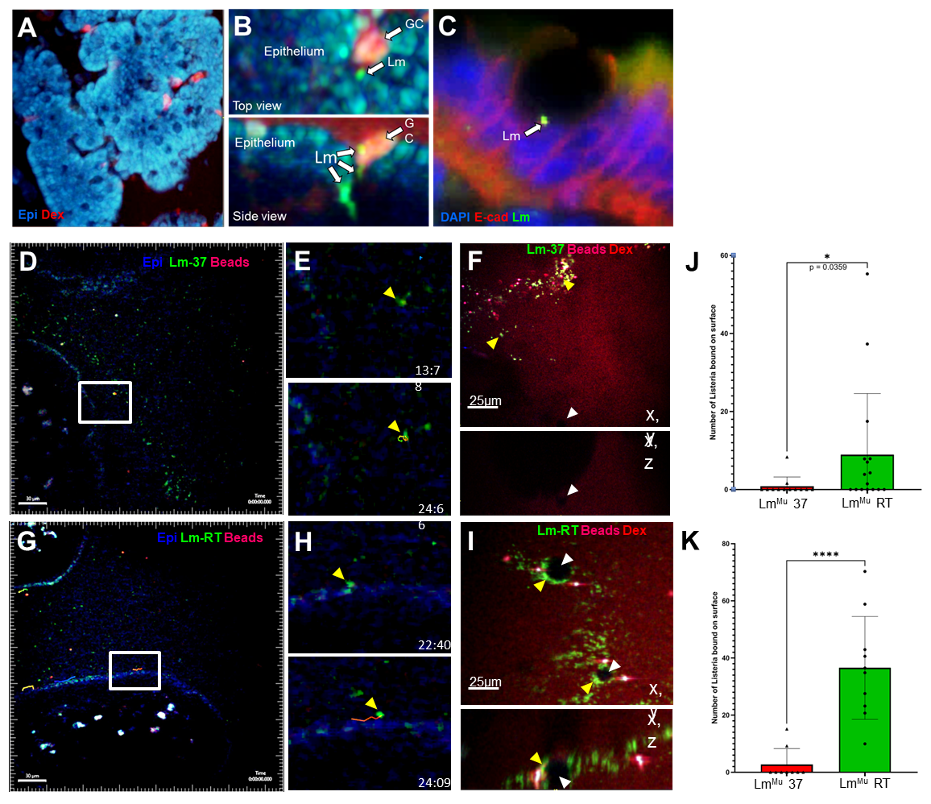
\includegraphics[page=1]{../img/figure3.png}};
		%\node at (0,0) {\figf A};
	\end{scope}
		
	\begin{scope}[xshift=8cm,yshift=-7.1cm]
		%\draw[fill=black] (0,0) rectangle +(1.5,-1.05);
			\draw [-{latex[scale=2]},line width=1.2pt,white](0.15,-.5) -- +(0.2,0);
			\node[white,anchor=west] at (0.3,-.5){\tiny GC};
			\draw [-{latex[scale=2]},line width=1.2pt,yellow](0.15,-.8) -- +(0.2,0);
			\node[yellow,anchor=west] at (0.3,-.8){\tiny Lm-RT};
		%\node at (0,0) {\figf A};
	\end{scope}
		
	\begin{scope}[xshift = 11.7cm, yshift=0cm]
		\node at (0,0) {\includegraphics{../plots/panelsJK.pdf}};
		\node at (0,-0.2) {\figf J};
		\node at (0,-4.8) {\figf K};
	\end{scope}

\end{tikzpicture}

\end{document}